\documentclass[
  bibliography=totoc,     % Literatur im Inhaltsverzeichnis
  captions=tableheading,  % Tabellenüberschriften
  titlepage=firstiscover, % Titelseite ist Deckblatt
]{scrartcl}


%synctex für inverses editieren
\synctex=1

% Grafiken können eingebunden werden
\usepackage{graphicx}
% größere Variation von Dateinamen möglich
\usepackage{grffile}
%relativer Pfad Grafiken nur mit Namen einbinden
\graphicspath{ {./abbildungen/}{./plots/} }

% kleine Verbesserungen des typesettings
\usepackage{microtype}

% code mit syntax highlighting
\usepackage{listings}

% LaTeX2e korrigieren.
\usepackage{fixltx2e}
% Warnung, falls nochmal kompiliert werden muss
\usepackage[aux]{rerunfilecheck}

% deutsche Spracheinstellungen
\usepackage{polyglossia}
\setmainlanguage{german}

% unverzichtbare Mathe-Befehle
\usepackage{amsmath}
% viele Mathe-Symbole
\usepackage{amssymb}
% Erweiterungen für amsmath
\usepackage{mathtools}

% Fonteinstellungen
\usepackage{fontspec}
\defaultfontfeatures{Ligatures=TeX}

\usepackage[
  math-style=ISO,    % \
  bold-style=ISO,    % |
  sans-style=italic, % | ISO-Standard folgen
  nabla=upright,     % |
  partial=upright,   % /
    warnings-off={           % ┐
      mathtools-colon,       % │ unnötige Warnungen ausschalten
      mathtools-overbracket, % │
    },                       % ┘
]{unicode-math}

\setmathfont{Latin Modern Math}
\setmathfont{xits-math.otf}[range={scr, bfscr}]
\setmathfont{xits-math.otf}[range={cal, bfcal}, StylisticSet=1]


% make bar horizontal, use \hslash for slashed h
\let\hbar\relax
\DeclareMathSymbol{\hbar}{\mathord}{AMSb}{"7E}
\DeclareMathSymbol{ℏ}{\mathord}{AMSb}{"7E}

% richtige Anführungszeichen
\usepackage[autostyle]{csquotes}

% Zahlen und Einheiten
\usepackage[
  locale=US,                   % deutsche Einstellungen
  separate-uncertainty=true,   % Immer Fehler mit \pm
  per-mode=symbol-or-fraction, % m/s im Text, sonst Brüche
  output-decimal-marker=.      % Punkt statt Komma
]{siunitx}

% chemische Formeln
\usepackage[
  version=4,
  math-greek=default, % ┐ mit unicode-math zusammenarbeiten
  text-greek=default, % ┘
]{mhchem}

% schöne Brüche im Text
\usepackage{xfrac}

% Floats innerhalb einer Section halten
\usepackage[section, below]{placeins}
% Captions schöner machen.
\usepackage[
  labelfont=bf,        % Tabelle x: Abbildung y: ist jetzt fett
  font=small,          % Schrift etwas kleiner als Dokument
  width=0.9\textwidth, % maximale Breite einer Caption schmaler
]{caption}
% subfigure, subtable, subref
\usepackage{subcaption}


% Standardplatzierung für Floats einstellen
\usepackage{float}
\floatplacement{figure}{htbp}
\floatplacement{table}{htbp}

% schöne Tabellen
\usepackage{booktabs}

% Seite drehen für breite Tabellen
\usepackage{pdflscape}

% Literaturverzeichnis
\usepackage{biblatex}
% Quellendatenbank
\addbibresource{lit.bib}
\addbibresource{programme.bib}

% Hyperlinks im Dokument
\usepackage[
  unicode,
  pdfusetitle,    % Titel, Autoren und Datum als PDF-Attribute
  pdfcreator={},  % PDF-Attribute säubern
  pdfproducer={}, % "
]{hyperref}
% erweiterte Bookmarks im PDF
\usepackage{bookmark}

% Trennung von Wörtern mit Strichen
\usepackage[shortcuts]{extdash}

\setmathfont{texgyretermes-math.otf}

\author{
  Philipp Hoffmann%
  \texorpdfstring{
    \\
    \href{mailto:philipp2.hoffmann@udo.edu}{philipp2.hoffmann@udo.edu}
  }{}%
  \texorpdfstring{\and}{, }
  Alexander Drossel 
  \texorpdfstring{
    \\
    \href{mailto:alexander.drossel@udo.edu}{alexander.drossel@udo.edu}
  }{}
}
\publishers{TU Dortmund – Fakultät Physik}


\newcommand{\bra}[1]{\langle #1 \rvert}
\newcommand{\ket}[1]{\lvert #1 \rangle}
%\newcommand{\liminf}[1]{\lim _{ #1 \to \infty} }
\newcommand{\dd}[2]{\frac{\mathrm{d} #1 }{\mathrm{d} #2 } }
\newcommand{\ddd}[2]{\frac{\mathrm{d}^2 #1}{\mathrm{d} #2 ^2} }
\newcommand{\pp}[2]{\frac{\mathrm{\partial} #1 }{\mathrm{\partial}#2 } }
\newcommand{\ppp}[2]{\frac{\mathrm{\partial}^2 #1 }{\mathrm{\partial} #2 ^2} }
\newcommand{\rvec}{\vec{r}}
\newcommand{\xvec}{\vec{x}}
\newcommand{\pvec}{\vec{p}}
\newcommand{\kvec}{\vec{k}}
\newcommand{\vvec}{\vec{v}}
%\newcommand{\dV}{\mathrm{d}V}
%\newcommand{\dA}{\mathrm{d}A}
%\newcommand{\dr}{\mathrm{d}r}
%\newcommand{\drvec}{\mathrm{d}\vec{r}}
%\newcommand{\dx}{\mathrm{d}x}
%\newcommand{\dy}{\mathrm{d}y}
%\newcommand{\dz}{\mathrm{d}z}
%\newcommand{\dt}{\mathrm{d}t}
%\newcommand{\dphi}{\mathrm{d}\phi}
%\newcommand{\dtheta}{\mathrm{d}\theta}
%\newcommand{\domega}{\mathrm{d}\omega}
%\newcommand{\rezi}[1]{\frac{1}{#1}
%\newcommand{\psirt}{\psi (\vec{r}, t)}
%\newcommand{\psirtav}{|\psi (\vec{r}, t)|^2}
\newcommand{\intzi}{\int _0 ^\infty}
\newcommand{\intii}{\int _{-\infty} ^\infty}
%\newcommand{\intmii}{\int _\infty ^\infty}
%\newcommand{\intmizero}{\int _\infty ^\infty}

%%% Hier definiert man Titel, Autor und Datum %%%%%%%%%%%%%%%%%%%%%%%%%%%%%%%%%

\subject{E5b Lehrstuhlversuch}
\title{Datenanalyse mit IceCube-Monte-Carlo Simulationsdaten}
\date{
  Durchführung: 14.09.2016
  \hspace{3em}
  Abgabe: 22.09.2016
}
%%%%%%%%%%%%%%%%%%%%%%%%%%%%%%%%%%%%%%%%%%%%%%%%%%%%%%%%%%%%%%%%%%%%%%%%%%%%%%%

\begin{document}

\maketitle
\thispagestyle{empty}
\tableofcontents
\newpage

\section{Einleitung}
\label{sec:Theorie}
\subsection{Ziel des Versuchs}
\label{sec:Ziel}
Ziel des Versuchs ist es anhand simulierter Daten des Ice-Cube-Experiments die relevanten Signale mittels maschinellen Lernens vom Untergrund zu trennen.
Hierbei liegt der Fokus auf den einzelnen Schritten, die für die Trennung der Daten durchlaufen werden.
Es sollen so Grundkenntnisse über das maschinelle Lernen am Ice-Cube-Experiment aufgezeigt werden.

\subsection{Astrophysikalische Grundlagen}
\label{sec:GrundlagenATP}
Im Jahre 1912 wurde erstmals von Viktor Heß die Höhenstrahlung entdeckt.
Seitdem ist bekannt, dass nicht nur Photonen in die Atmosphäre der Erde eindringen, sondern auch Protonen und schwerere Kerne.
Dies wird als Höhenstrahlung bzw. geladene kosmische Strahlung bezeichnet.
Bei der geladenen Strahlung werden Energien von bis zu $\SI{e20}{\electronvolt}$ beobachtet und sie folgt annähernd einem Potenzgesetz
\begin{align*}
	\frac{\mathrm{d}\theta}{\mathrm{d}E} = \theta _0 E^\gamma
\end{align*}
mit $\gamma \approx -\SI{2.7}{}$ als dem spektralen Index.
Geladene kosmische Strahlung besteht zum Großteil aus Protonen und geladenen Kernen und wird durch (extra)galaktische Magnetfelder abgelenkt.
Deswegen lässt sich die Quelle dieser Strahlung nicht ermitteln.
Jedoch sollten Quellen die Hadronen beschleunigen, auch Neutrinos und hochenergetische Photonen erzeugen.
Da Neutrinos im Gegensatz zu hadronischen Teilchen ungeladen sind und einen sehr kleinen Wirkungsquerschnitt besitzen, werden sie nicht von Magnetfeldern abgelenkt und können durch die sehr selten auftretenden Wechselwirkungen zu einem deutlich größeren Anteil Materie durchdringen.
Neutrinos zeigen somit nahezu direkt auf ihren Ursprungsort zurück. 
%Der Spektrale Index von Neutrinos wird mit $\gamma \approx -2$ angegeben.

\subsection{Das IceCube-Experiment}
\label{sec:eiswürfel}
Das IceCube-Experiment am geografischen Südpol dient zur Detektion hochenergetischer Neutrinos.
Es besteht aus drei Stationen: IceTop, dem In-Ice-Array und DeepCore.
Das In-Ice-Array und DeepCore bestehen aus 86 in Eis eingeschmolzenen Kabeln, an denen in einer Eistiefe von $\SI{1450}{m}$ bis $\SI{2450}{m}$ insgesamt $\SI{5160}{}$ Photoelektronenvervielfachern angebracht sind.
Davon befinden sich sieben Kabel mit einem geringeren Abstand aneinander und bilden so den DeepCore.
DeepCore besitzt eine untere Energieschwelle von $\SI{10}{\giga\electronvolt}$.
Die Energieschwelle des restlichen In-Ice-Arrays liegt bei $\SI{100}{\giga\electronvolt}$.
An der Oberfläche des Eises befindet sich das Luftschauer-Experiment IceTop.
Hier werden die Teilchen in lichtdichten Eistanks über ihr Tscherenkowlicht detektiert.
Da sich IceTop an der Oberfläche befindet kann diese Station als Veto für die Neutrinodetektion verwendet werden, weil hier hauptsächlich kosmische Strahlung und Teilchen aus Luftschauern in Wechselwirkung treten.
So ist es beispielsweise auch möglich Neutrinos vom Südhimmel zu detektieren.
Tscherenkowlicht entsteht, wenn sich geladene Teilchen schneller als Lichtgeschwindigkeit in einem Medium bewegen.
Im Eis werden die Neutrinos der Flavour $\ell$ mittels Sekundärteilchen detektiert.
Diese entstehen durch die zwei folgenden Wechselwirkungen mit Kernen $A$ im Eis und restlichen Reaktionsprodukten $X$:
\begin{align*}
	\nu_\ell(\bar{\nu_\ell}) + A \rightarrow \ell^{\pm} + X \\
	\nu_\ell + A \rightarrow \nu_\ell + X
\end{align*}
Da Myonen eine Vergleichsweise lange Lebensdauer besitzen werden diese und ihre Erzeuger, die Myon-Neutrinos, am häufigsten detektiert.
Myonen aus Neutrinointeraktionen sind im Folgenden das Signal.
Jedoch werden Myonen auch in großer Zahl durch Wechselwirkung geladener kosmischer Strahlung in der Atmosphäre erzeugt; diese sind der Untergrund.
\begin{align*}
	p + A \rightarrow \pi^+/K^+ + X, \\
	\pi^+/K^+\rightarrow \mu + \nu_{\mu}.
\end{align*}
Myonen aus Luftschauern treten ca. $\SI{e6}{}$-mal so häufig auf wie Myonen aus Myon-Neutrinos.
Da Myonen im Gegensatz zu Neutrinos nicht die Erde durchqueren können, muss es sich bei Ereignissen deren rekonstruierte Richtung nicht vom Südhimmel kommt um Neutrinos oder fehlrekonstruierte kosmische Myonen handeln.
Wird so ein Schnitt am Zenitwinkel der rekonstruierten Richtung durchgeführt bleiben noch etwa $\SI{e3}{}$-mal so viele Untergrund- wie Signalereignisse.
Um diese vom Signal zu trennen werden Methoden des maschinellen Lernens verwendet.

\section{Methoden des maschinellen Lernens}
\label{sec:mashlearning}

Um die relevanten Signale von den Untergrunddaten zu trennen werden in diesem Versuch Methoden des maschinellen Lernens verwendet.
Der typische Ablauf für die Prozessierung simulierter Daten sieht wie folgt aus:
\begin{description}

\item[Vorbereitung der Daten] Zu Beginn werden die Daten für die weiteren Schritte vorbereitet.
\item[Attributselektion] Es werden die für die Lerner relevanten Attribute mit einem Algorithmus herausgesucht. 
Dies verringet die Rechenzeit in den folgenden Schritten drastisch.
Die Attributselektion wird hiernach mit dem Jaccard-Index auf die Stabilität gegen statistische Schwankungen im Lerner untersucht.
\item[Multivariate Selektion] Die Lernen werden auf die vorbereiteten Datensätze trainiert. 
Der trainierte Lerner lässt sich danach auf andere Datensätze anwenden.
\item[Überprüfen der prozessierten Daten] Zum Schluss werden die bearbeiteten Daten auf ihre Genauigkeit geprüft. 
Hierzu werden Qualitätsparameter eingeführt und die Lerner mittels Kreuzvalidierung getestet.

\end{description}

Im Folgenden werden diese Schritte und einige der in diesem Versuch verwendeten Methoden näher erläutert.

\subsection{Attributsselektion mittels mRMR}
\label{sec:mRMR}

Bei der Attributsauswahl mittels minimum Redundancy Maximum Relevance (mRMR) wird die Wahrscheinlichkeitsverteilung der einzelnen Attribute betrachtet und ist somit nicht von einem spezifischen Lerner abhängig.
Hierzu wird der wechselseitige Informationsgehalt zweier Attribute $x$, $y$ benutzt:
\begin{align*}
	I(x,y)=\int p(x,y)\log \left( \frac{p(x,y)}{p(x)p(y)}  \right)\textrm{d}x\textrm{d}y
\end{align*}
Hierbei bezeichnen $p(x),\, p(y)$ und $p(x,y)$ die Wahrscheinlichkeitsdichtefunktionen der betreffenden Attribute. 
Die Attribute werden hierbei vom mRMR-Algorithmus so ausgewählt, dass sie möglichst stark mit dem Zielattribut, aber untereinander möglichst wenig korreliert sind.

\subsection{Stabilitätsanalyse mit dem Jaccard-Index}
\label{sec:jaccard}
Der Jaccard-Index in ein Maß für die Ähnlichkeit zweier Mengen.
Um ihn zu berechnen teilt man die Anzahl der gemeinsamen Elemente (Schnittmenge) durch die Größe der Vereinigungsmenge:
\begin{align*}
	J(A,B) = \frac{\vert A \cap B \vert}{\vert A \cup B \vert }
\end{align*}
Dies wird $l$-mal auf $l$ Teilmengen des Datensatzes angewendet. 
Somit lässt sich die Ähnlichkeit der verschiedenen Selektionen beurteilen.
Hierbei beschreibt ein Wert um $\SI{1.0}{}$ eine maximal stabile Attributauswahl gegen statistische Schwankungen.
\begin{align*}
	\hat{J} = \frac{2}{l(l-1)} \sum_{i=1}^l \sum_{j=i+1}^l J(F_i,F_j)
\end{align*}


\subsection{Multivariate Lerner}
\label{sec:multilearn}
Die Verwendung von multivariaten Lernern bietet den Vorteil, dass diese auch Korrelationen zwischen den Variablen beachten.

\subsubsection{Random Forest}
\label{sec:rndforest}
Der Random Forest Lerner basiert auf binären Entscheidungsbäumen. 
Jeder Entscheidungsbaum erhält nur eine Teilmenge der vorhandenen Attribute oder Ereignisse, womit die Korrelation der Bäume untereinander verkleinert wird.
Beim erstellen eines solchen Baums werden für jedes Ereignis an den Knoten die Werte eines Attributs betrachtet. 
Es wird durch Minimieren oder Maximieren eines Optimierungskriteriums ein Schnitt in diesem Attribut gesetzt.
Diese Schnitte werden wiederholt, bis die maximale Tiefe des Baums erreicht ist.
Der letzte Attributsschnitt bestimmt zu welcher Klasse ein Ereignis zugeordnet wird.
Beim vorliegenden Zweiklassenproblem dieses Versuchs ist dies entweder Signal oder Untergrund, was als 1 oder 0 ausgedrückt werden kann.
Um den Effekt des Übertrainings zu minimieren, werden $N$ Bäume angelegt und folgend über diese zu einer Konfidenz gemittelt. 
Die Konfidenz (c) des Random Forest-Algorithmus wird definiert als das Mittel über der Entscheidungen $P_i$ der $N$ Teilbäume:
\begin{align*}
	c= \frac{1}{N}\sum_{i=1}^NP_i, P_i \in \{0,1\}
\end{align*}

\subsubsection{Naive Bayes-Algorithmus}
\label{sec:dernaivebayes}

Der Naive-Bayes-Algorithmus basiert auf dem Satz von Bayes.
Dies ist ein mathematischer Satz der Wahrscheinlichkeitstheorie, der die Berechnung bedingter Wahrscheinlichkeiten beschreibt.
Die bedingte Wahrscheinlichkeit $P(A \vert B)$ ist die (bedingte) Wahrscheinlichkeit, dass Ereignis $A$ eintritt, unter der Bedingung, dass $B$ bereits eingetreten ist.
Das Bayes'sche Theorem sagt aus:
\begin{align*}
	p(A \vert B) = \frac{p(B\vert A)p(A)}{p(B)}
\end{align*}
In diesem Fall beschreibt A die Klassenzugehörigkeit (Signal $A$ oder Untergrund $\bar{A}$) und B ein Attribut. 
Somit lässt sich folgender Ausdruck Formulieren:
\begin{align*}
	Q = \frac{p(A \vert B)}{p(\bar{A}\vert B)}=\frac{p(B \vert A)p(A)}{p(B \vert \bar{A})p(\bar{A})}
\end{align*}
Dieser Ausdruck nimmt einen Wert von 1 an, wenn das Ereignis mit höherer Wahrscheinlichkeit ein Signal ist.
Für mehrere Attribute wird der Ausdruck zu:
\begin{align*}
	Q = \frac{p(A \vert B_1,...,B_n)}{p(\bar{A}\vert B_1,...,B_n)}=\prod_{i=1}^n \frac{p(B_i \vert A)}{p(B_i \vert \bar{A})}
\end{align*}

\subsection{Gradient Boosting}
\label{sec:gradient}

Gradient Boosting ist ein iterativer Lerner der auf Entscheidungsbäumen basiert.
Er erzeugt in jedem Iterationsschritt einen neuen Lerner, der eine möglichst geringe Abweichung zum idealen Modell besitzen soll.
Dies geschieht durch Minimierung einer Kostenfunktion, welche anhand der Start-/ und Zielwerte, sowie dem vorangegangenen Lerner, ein Maß für die Abweichung der durch den Lerner errechneten Zielwerte zu den realen Zielwerten beschreibt.
Diese Lerner können alleine betrachtet als schwach bezeichnet werden und stellen noch kein gutes Modell dar.
Beim Gradient Boosting wird mit den in den Iterationsschritten berechneten Gewichten und zugehörigen schwachen Lernern eine gewichtete Summe gebildet.
Das Ergebnis dieser kann somit als ein starker Lerner bezeichnet werden.



%testrebase

\subsection{Qualitätsparameter}
\label{sec:quali}
Um die Güte der Entscheidungen eines Lerners zu berechnen werden Qualitätsparameter eingeführt.
\begin{align}
    \textrm{Reinheit  } p &= \frac{\mathrm{tp}}{\mathrm{tp}+\mathrm{fp}} \\
    \textrm{Effizienz  } r &= \frac{\mathrm{tp}}{\mathrm{tp}+\mathrm{fn}}
\end{align}
Mit dem richtig als Signal klassifizierten Ereignissen ($\mathrm{tp}$, true positive), den richtig als Untergrund klassifizierten Ereignissen ($\mathrm{tn}$, true negative) und der Anzahl der fälschlich als Signal ($\mathrm{fp}$, false positive) bzw. fälschlich als Untergrund ($\mathrm{fn}$, false negative) klassifizierten Ereignisse.






%\begin{figure}
    %\begin{subfigure}{.5\textwidth}
%  \centering
%  \includegraphics[width=0.80\textwidth]{}
%  \caption{.}
%  \label{fig1}
%\end{subfigure}
%\end{figure}

\section{Durchführung}
\label{sec:Durchführung}

In diesem Teil wird auf die verwendeten Methoden des maschinellen Lernens eingegangen sowie die Vorprozessierung der Daten erläutert.
Für diesen Versuch werden simulierte Signal- und Untergrundereignisse verwendet. 
Für den Vergleich zwischen den verschiedenen Lernen werden drei verschiedene Lerner verwendet.


\subsection{Vorprozessierung}
\label{sec:vorprozessierung}

Der Zweck der Vorprozessierung ist es die Signal- und Untergrunddaten in einen gemeinsamen Datensatz zu bringen und nicht sinnvoll verwendbare Attribute zu entfernen. 
Hierzu müssen alle Attribute entfernt werden die nicht in beiden Datensätzen vorkommen. 
Weiterhin werden alle Monte-Carlo-Wahrheiten und Werte die nicht als Zahl identifiziert werden können (NaN, Inf) entfernt oder ersetzt. 
Als letztes werden die Daten mit einem binären Label versehen, das bestimmt ob ein Ereignis zu Signal und Untergrund gehört und das als Zielattribut für die Lerner verwendet wird. 


\subsection{Attributselektion}
\label{sec:attselection}

Um die Rechenzeit zu verringern ist es sinnvoll zuerst die Attribute auszuwählen, die dem Lerner eine möglichst gute Unterscheidung zwischen Signal und Untergrund ermöglichen. 
Für diesen Prozess gibt es mehrere Verfahren, darunter die Vorwärtsauswahl (Forward Selection) und die mRMR-Auswahl (minimum Redundancy, Maximum Relevance). 
Die Vorwärtsauswahl gibt das bestmögliche Ergebnis, besonders weil es Attribute auswählt die für einen bestimmten Lerner am besten sind, was dafür sorgt, dass die Attributsauswahl nicht verallgemeinerbar ist.
Die Vorwärtsauswahl ist außerdem mit einer sehr hohen Rechenzeit verbunden und erhöht durch das oft wiederholte Trainieren des Lerners die Gefahr der Überanpassung des Modells an die vorhandenen Daten.

Aus diesem Grund wird in diesem Versuch die mRMR-Auswahl verwendet. 
Siehe hierzu Kapitel \ref{sec:mRMR}.
Um die Stabilität der Attributauswahl gegen statistische Schwankungen zu testen wird hierbei der Jaccard-Index verwendet, siehe Kapitel \ref{sec:jaccard}.


\subsection{Lernalgorithmen}
\label{sec:lernalgo}

In diesem Versuch wird als Lerner der RandomForest-Algorithmus (Kapitel \ref{sec:rndforest}), Gradient Boosting (Kapitel \ref{sec:gradient}) und der Naive Bayes-Algorithmus (Kapitel \ref{sec:dernaivebayes}), verwendet. 
Sie werden in einer Kreuzvalidierung trainiert , um zu zeigen, dass der Lerner auch auf Datensätze angewendet werden kann auf die er nicht trainiert wurde. 
Hierzu wird der Datensatz in $n$ Teile aufgeteilt und auf $n-1$ von diesen trainiert. Daraufhin wird er auf den letzten Datensatz angewendet um den Lerner zu validieren. 
Das Vorgehen wird $n$-mal wiederholt, sodass jeder Datensatz einmal zum testen verwendet wird. 
Zum Überprüfen der Qualität des Lerners werden die Qualitätsparameter aus Kapitel \ref{sec:quali} verwendet.









%\begin{figure}
    %%\begin{subfigure}{.5\textwidth}
  %\centering
  %\includegraphics[width=0.80\textwidth]{}
  %\caption{.}
  %\label{fig1}
%%\end{subfigure}
%\end{figure}

\section{Auswertung}
\label{sec:Auswertung}
Die Auswertung hat den Vergleich mehrerer Algorithmen des maschinellen Lernens zum Ziel.
Dafür werden die zur Verfügung gestellten Daten erst mit Pandas~\cite{pandas} vorprozessiert und auf ihnen mittels mRMR~\cite{mrmre} eine Attributselektion durchgeführt.

\subsection{Vorprozessierung}
Die zur Verfügung gestellten Datensätze bestehen aus insgesamt $\num{40000}$ Ereignissen.
Eine Hälfte davon sind Neutrinos (Signal), die andere Myonen (Untergrund).
Von diesen Ereignissen werden zuerst Attribute entfernt, die nicht in beiden Datensätzen vorhanden sind; es bleiben 237 Attribute übrig.
Dann werden unphysikalische Attribute, wie die IDs der Ereignisse und Informationen, die nur in der Simulation vorhanden sind, entfernt; es bleiben 188 Attribute übrig.
Dann werden Attribute mit einem Anteil an NaN-Werten von über 20\% entfernt; es bleiben 169 Attribute übrig.
Basis dafür ist die NaN-Verteilung in Abbildung~\ref{nanverteilung}.
Sie zeigt, dass die meisten Attribute weniger als 20\% NaNs enthalten.
Die etwa 19 Attribute mit einem Anteil größer 90\% enthalten nicht genügend Informationen für die Separation.
Die NaNs in den restlichen Attributen werden durch die Zahl -5000 ersetzt.
Eigentlich könnten alle NaNs auch zuerst mit dieser Zahl ersetzt werden und das Ausfiltern der Attribute mit zu vielen NaNs der Attributselektion überlassen werden.
Sind zu viele NaNs vorhanden entspricht dies einem geringen Informationsgehalt des Attributs, was automatisch erkannt werden sollte.
Konstante Attribute wurden auch nicht explizit entfernt, da diese vom mRMR automatisch herausgefiltert werden.
\begin{figure}
  \centering
  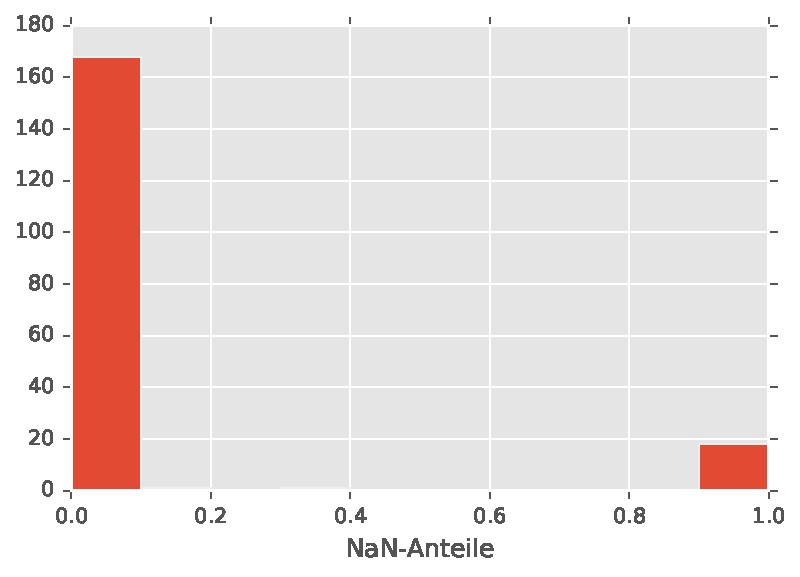
\includegraphics[width=0.80\textwidth]{nanplot}
\vspace{-1em}
  \caption{Histogramm der NaN-Anteile in den noch vorhandenen Attributen.}
  \label{nanverteilung}
\end{figure}


\subsection{Attributselektion}
Durchgeführt wird eine fünffache Attributselektion mittels mRMR.
Dafür werden aus der Menge der Gesamtereignisse fünf gleich große Ereigismengen mit zurücklegen gezogen und auf jeder dieser Mengen eine Attributselektion durchgeführt, um so eine Abschätzung der Varianz der Selektion zu erhalten. 
Die dafür verwendeten Ereignismengen wurden durch Ziehen mit Zurücklegen aus der Gesamtmenge von $\num{40000}$ Ereignissen erstellt.
Als Stabilität der Attributselektion wird der Jaccard-Index verwendet.
Die gemittelten Stabilitäten mit ihren Standardabweichungen gegen die Anzahl an selektierten Attributen $k$ sind in Abbildung~\ref{jaccardplot} zu sehen.
Die Mittelwerte steigen erst und sättigen sich bei $k=28$ zu etwa 0.9.
Hier ist auch die Standardabweichung der Mittelwerte am kleinsten.
Dieser $k$-Wert wird als Zahl der Attribute für die Separation gewählt.
Welche 28 Attribute genau ausgewählt werden, wird über eine eine Mehrheitsentscheidung der fünf Attributselektionen bestimmt.
Die 28 Attribute, die im Durchschnitt der Selektionen die höchsten Bewertungen erhalten, werden ausgewählt.
\begin{figure}
  \centering
  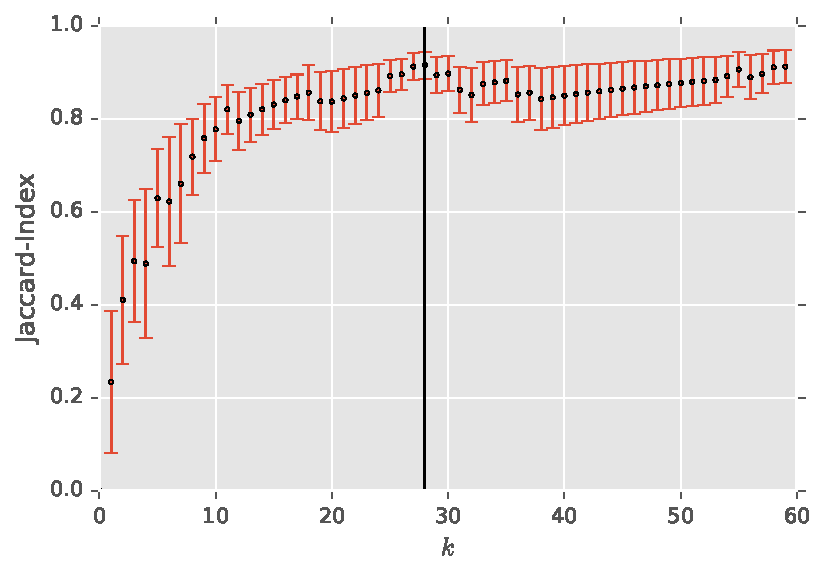
\includegraphics[width=0.80\textwidth]{jaccard}
\vspace{-1em}
  \caption{Die Mittelwerte der Jaccard-Indices mit ihren Standardabweichungen, gegen die Anzahl an selektierten Attributen.}
  \label{jaccardplot}
\end{figure}


\subsection{Separation}
Für die Separation werden innerhalb der Optimierung durch auto-sklearn~\cite{autosklearn} Algorithmen aus scikit-learn~\cite{scikit-learn} verwendet.
Außerdem wird noch der Naive-Bayes und Gradient Boosted Trees Operator aus RapidMiner~\cite{RapidMiner}, sowie der WEKA Random Forest~\cite{Weka2009} verwendet.


\subsubsection{Naive-Bayes}
Als Referenz für die Separationsqualitäten wurde der Naive-Bayes (NB) Algorithmus betrachtet.
Die gemittelten Reinheiten und Effizienzen aus der Kreuzvalidierung gegen die Konfidenz sind in Abbildung~\ref{naivebayes} zu finden.
Die Standardabweichungen des Mittelwerts sind als transparentes Band um die Mittelwerte eingezeichnet.
Der NB zeigt bereits eine sehr starke Trennung der beiden Klassen.
Die Reinheit steigt für größer werdende Konfidenzen nur in einem einstelligen Prozentbereich und erreicht einen maximalen Wert nahe 1.
Die Standardabweichungen sind im Verhältnis zu den Mittelwerten vernachlässigbar klein.
\begin{figure}
  \centering
  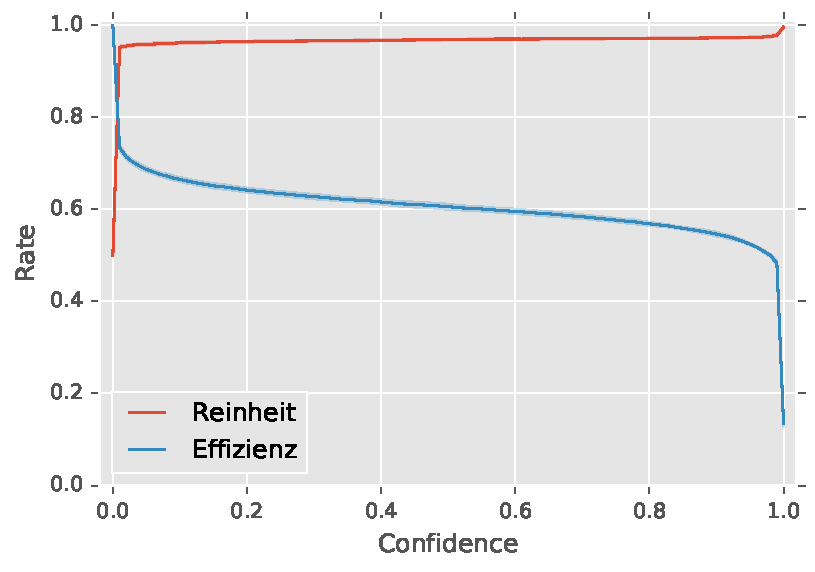
\includegraphics[width=0.80\textwidth]{bayesquality}
\vspace{-1em}
    \caption{Aufgetragen sind Mittelwerte der Reinheiten und Effizienzen mit ihren Standardabweichungen (als farbige Bänder) gegen die Konfidenz für den Naive-Bayes aus einer fünffachen Kreuzvalidierung.}
  \label{naivebayes}
\end{figure}

\subsubsection{Random Forest}
Der Random Forest wurde mit RapidMiner mit 200 Bäumen und dem Entropie Optimierungskriterium auf $\num{40000}$ Ereignissen trainiert.
Die Reinheit und Effizienz gegen die Konfidenz des Random Forests ist in Abbildung~\ref{figrndforestquality} dargestellt.
Der Random Forest zeigt ab Konfidenzen größer 0.5 eine höhere Reinheit als auch Effizienz als der NB.
Bei einer Konfidenz von 1.0 holt der NB in der Reinheit auf, während die Effizienz um etwa 25\% schlechter wird.
Die Standardabweichungen sind im Verhältnis zu den Mittelwerten vernachlässigbar klein.
\begin{figure}
  \centering
  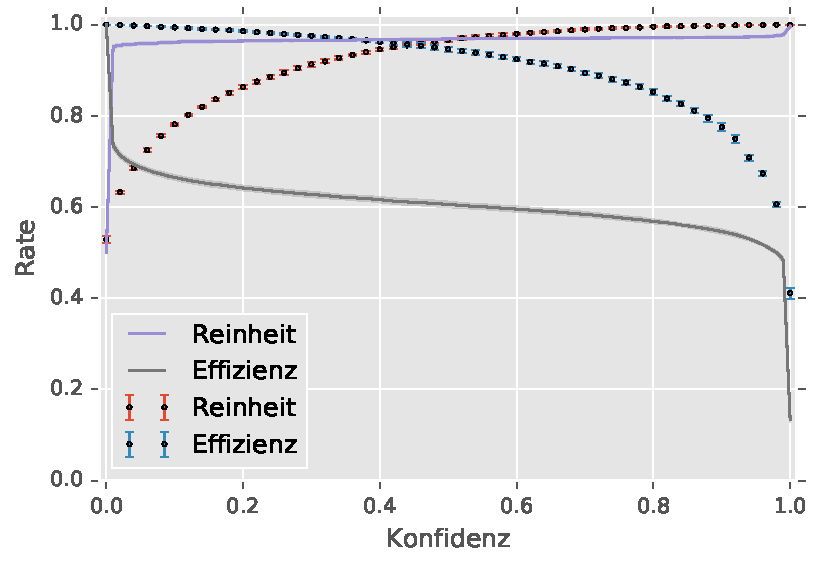
\includegraphics[width=0.80\textwidth]{rndforestquality}
\vspace{-1em}
    \caption{Aufgetragen sind Mittelwerte der Reinheit und Effizienz mit ihren Standardabweichungen gegen die Konfidenz für den Random Forest (Punkte) und den Naive-Bayes (durchzogene Linien) aus einer fünffachen Kreuzvalidierung. Die Standardabweichungen sind durch die farbigen Bänder und Fehlerbalken gekennzeichnet.}
  \label{figrndforestquality}
\end{figure}



\subsubsection{Gradient Boosting}
Die Algorithmenauswahl und Hyperparameterbestimmung erfolgt durch die Python Bibliothek auto-sklearn~\cite{autosklearn}, die ein Ensemble aus mehreren Lernern erstellt und ihre Hyperparameter anhand von selbst auswählbaren Qualitätskriterien optimiert.
Als zu maximierendes Kriterium wurde die der Anteil richtig Klassifizierter Ereignisse an der Gesamtmenge der Ereignisse gewählt.
Die zu verwendenden Algorithmen wurden über 27 Stunden optimiert.
Dabei hat auto-sklearn zuerst ein Gemisch aus Random Forests, Gradient Boosting und anderen Methoden verwendet.
Nach mehreren Stunden Rechenzeit wurden alle Algorithmen durch eine Kombination von 20 Gradient Boosting Lernern ersetzt.

Reinheit und Effizienz mit ihren Standardabweichungen gegen die Konfidenz sind in Abbildung~\ref{figaskquality} zu sehen.
Der Durchschnitt der Konfidenzen der einzelnen Lerner ist die Konfidenz des Ensembles.
Die Effizienz des auto-sklearn Ensembles ist für alle Konfidenzen außer 1.0 höher als die des Naive-Bayes.
Für Konfidenzen größer 0.5 zeigen sich, wie beim Random Forest, höhere Reinheiten als beim NB.
Die Standardabweichungen sind im Verhältnis zu den Mittelwerten vernachlässigbar klein.
\begin{figure}
  \centering
  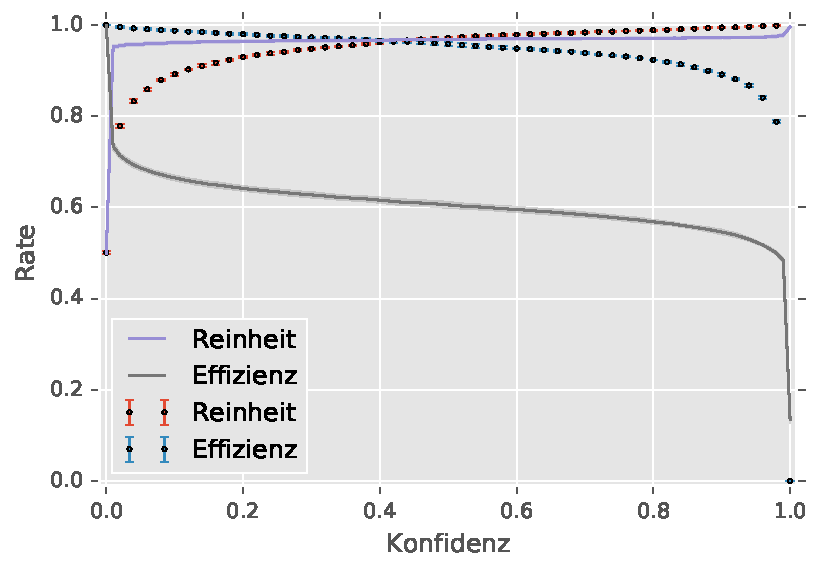
\includegraphics[width=0.80\textwidth]{askquality}
\vspace{-1em}
    \caption{Aufgetragen sind Mittelwerte der Reinheit und Effizienz mit ihren Standardabweichungen gegen die Konfidenz für das auto-sklearn ensemble (Punkte) und den Naive-Bayes (durchzogene Linien) aus einer fünffachen Kreuzvalidierung. Die Standardabweichungen sind durch die farbigen Bänder und Fehlerbalken gekennzeichnet.}
  \label{figaskquality}
\end{figure}

Abbildung~\ref{figrmgbquality} ist analog zu Abbildung~\ref{figaskquality} erstellt worden.
Es wurde hier das Gradient Boosting Ensemble von auto-sklearn durch den RapidMiner Gradient Boosted Trees Operator ersetzt.
Es zeigt sich ein sehr ähnliches Bild wie in Abbildung~\ref{figaskquality}.
\begin{figure}
  \centering
  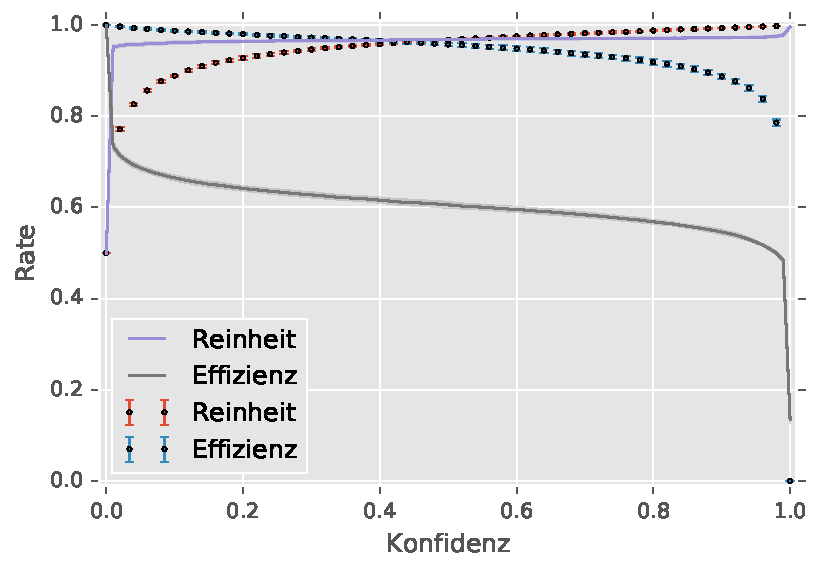
\includegraphics[width=0.80\textwidth]{rmgbquality}
\vspace{-1em}
    \caption{Aufgetragen sind Mittelwerte der Reinheit und Effizienz mit ihren Standardabweichungen gegen die Konfidenz für das den RapidMiner Gradient Boosted Trees Operator (Punkte) und den Naive-Bayes (durchzogene Linien) aus einer fünffachen Kreuzvalidierung. Die Standardabweichungen sind durch die farbigen Bänder und Fehlerbalken gekennzeichnet.}
  \label{figrmgbquality}
\end{figure}


\subsection{Vergleich der Gradient Boosted Trees}
Die Qualitätsunterschiede zwischen der RapidMiner Gradient Boosted Trees Implementierung und dem optimierten Ensemble von Gradient Boosted Trees aus auto-sklearn werden in Abbildung~\ref{figgbvsgb} in einem kleineren Ausschnitt verglichen.
Die durchzogenen Linien sind die Mittelwerte des auto-sklearn Ensembles.
Es zeigen sich nur geringe Abweichungen zwischen den beiden Lernern, die nur bei Konfidenzen um 0.5 größer als eine Standardabweichungen der beiden Lerner werden.
Die Lerner sind somit weitgehend äquivalent.
\begin{figure}
  \centering
  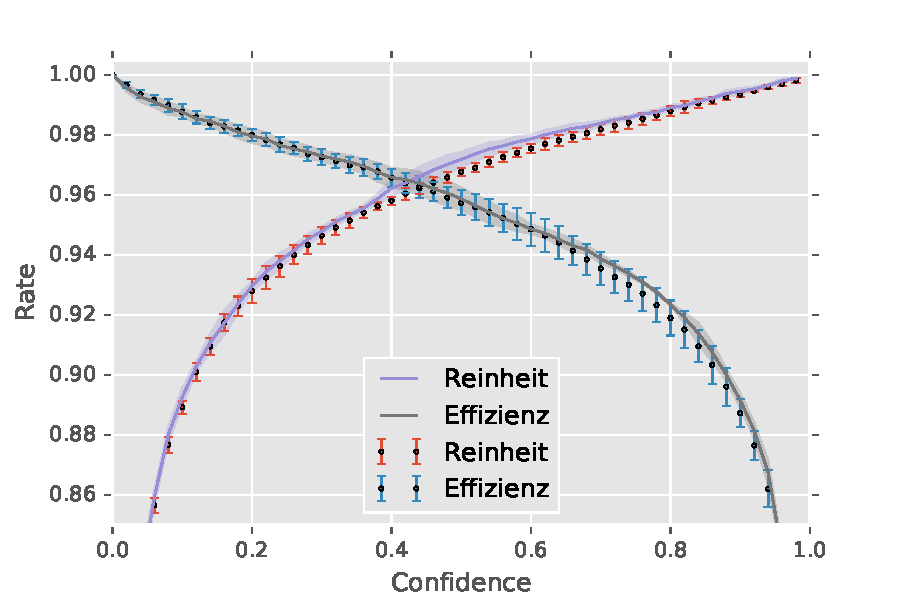
\includegraphics[width=0.80\textwidth]{gbvsgb}
\vspace{-1em}
    \caption{Aufgetragen sind Mittelwerte der Reinheit und Effizienz mit ihren Standardabweichungen gegen die Konfidenz für das auto-sklearn Ensemble (durchzogene Linien) und den RapidMiner Gradient Boosted Trees Operator (Punkte) aus einer fünffachen Kreuzvalidierung. Die Standardabweichungen sind durch die farbigen Bänder und Fehlerbalken gekennzeichnet.}
  \label{figgbvsgb}
\end{figure}


\subsection{Vergleich von Random Forest und Gradient Boosted Trees}
In Abbildung~\ref{figrfvsgb} wird der RapidMiner WEKA Random Forest Operator mit dem Gradient Boosted Trees (GBT) Operator verglichen.
Der GBT zeigt für alle Konfidenzen bis auf 1.0 eine höhere Effizienz, während für Konfidenzen größer 0.5 seine Reinheit leicht hinter der des Random Forests liegt.
Es ist zu beachten, dass für den GBT die Reinheiten für die selben Konfidenzen in diesem Bereich zwar niedriger als die des Random Forests sind, die Reinheiten des GBT für vorgegebene Werte der Effizienz aber höher als die des Random Forest sind.
Diese Überlegenheit des GBT gilt bis zu Reinheiten von 99.9\%, erst ab hier hat der GBT eine niedrigere Effizienz als der RF.
Die Effizienz des GBT wird dort gleich Null.
\begin{figure}
  \centering
  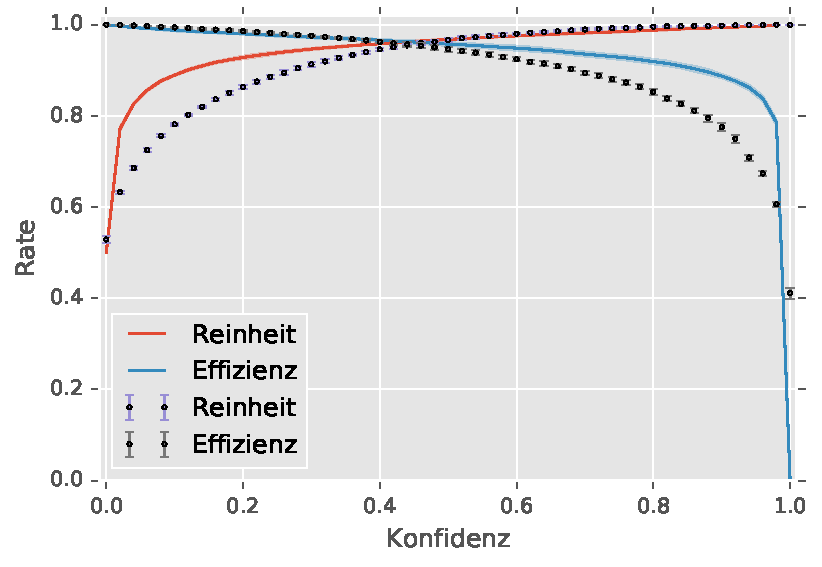
\includegraphics[width=0.80\textwidth]{rfvsgb}
\vspace{-1em}
    \caption{Aufgetragen sind Reinheit und Effizienz mit ihren Standardabweichungen gegen die Konfidenz für die RapidMiner Operatoren WEKA Random Forest (Punkte) und Gradient Boosted Trees (durchzogene Linien) aus einer fünffachen Kreuzvalidierung. Die Standardabweichungen sind durch die farbigen Bänder und Fehlerbalken gekennzeichnet.}
  \label{figrfvsgb}
\end{figure}






%oder einfach /input textable table
%\begin{table}
    %\sisetup{separate-uncertainty=true}
    %\centering
    %\caption{.}
    %\label{tab:1}
    %%\sisetup{table-format=2.1}
    %\begin{tabular}{l@{}S[table-format=-1.2, table-figures-uncertainty=1] S S S S}
        %\toprule
%%        & \multicolumn{2}{c}{Technetium} & \multicolumn{2}{c}{Molybdän} \\
        %%{} &
        %{\( /\si{} \)}  &  {\( /\si{} \)}  &  {\( /\si{} \)}  &  {\( /\si{} \)} \\
        %\midrule \input{messwerte/}
        %\bottomrule
    %\end{tabular}
%\end{table}

\section{Diskussion}
\label{sec:Diskussion}

In dieser Separation zeigen alle Lerner, selbst der Naive-Bayes, eine hohe Trennkraft, was für eine sehr gute Konstruktion der Attribute spricht.
Weiter zeigt sich, dass Gradient Boosted Trees für die vorliegenden Daten einem Random Forest überlegen sind, so lange nicht die bei einer Konfidenz von 1.0 auftretende höchstmögliche Reinheit gefordert wird.

Das auto-sklearn Ensemble aus 20 Gradient Boosted Tree Lernern zeigt trotz seines höheren Rechenaufwands nur geringe Abweichungen von der einfachen GBT Implementierung in Rapidminer.
Kann RapidMiner ohne weiteres Verwendet werden ist auto-sklearn den damit verbundenen Mehraufwand nicht wert.
Es bleibt jedoch offen, ob die Separation von auto-sklearn durch mehr Optimierungszeit verbesserbar ist, da hier etwa die hälfte der 27 Stunden gebraucht wurde um von verschiedenen Lernern auf ein Ensemble von Gradient Boosted Trees zu kommen, deren Einstellungen noch weiter angepasst werden können.


\printbibliography

\end{document}
